\documentclass{article} % Change the class here
\usepackage[T1]{fontenc}
\usepackage{minted}
\usepackage{seqsplit}
\usepackage{graphicx}

\begin{document}

\section{Exercise 1: Retrieving information for the protein TMM25\_HUMAN}

This code below does the following:

\begin{enumerate}
  \item Get the sequence (\verb+getSequence+)
  \item Split by lines (\verb+stream.splitlines()+)
  \item Trim all carriage returns (\verb+process+)
  \item Get the id (\verb+getid+)
  \item Get signal (\verb+get_signal_range+)
  \item Get sequence (\verb+get_aa_seq+)
\end{enumerate}

The output is: 

\begin{minted}[linenos=false,fontsize=\small]{text}
Currently processing the sequence with the name UNIPROT:TMM25_HUMAN
There is a signal peptide ending at  position 26
The signal peptide looks like this: MALPPGPAALRHTLLLLPALLSSGWG
\end{minted}

The code:

\begin{minted}[linenos=false,fontsize=\small]{python}
def exercise_1(query_seq: str):
    def process(txt):
        """make it a bit cleaner"""
        # return [[s.strip() for s in line.split(" ") if s] for line in txt]
        data = []
        for line in txt:
            data.append([s.strip() for s in line.split(" ") if s])
        return data

    def getid(lines):
        for line in lines:
            if line[0] == "ID":
                return line[1]

    def get_aa_seq(lines: list[list[str]], signal_start: int, signal_end: int):
        aa_start = 0
        aa_end = 0
        for lineno, line in enumerate(lines):
            if line[0] == "SQ":
                # everything from SQ to end is protein sequence
                aa_start = lineno
            if line[0] == "//":
                aa_end = lineno

        aa = "".join(
            [item for sublist in lines[aa_start + 1 : aa_end] for item in sublist]
        )
        # minus 1, lists start at 0
        return aa[signal_start - 1 : signal_end]

    def get_signal_range(lines: list[list[str]]) -> tuple[int, int]:
        for line in lines:
            if line[0] == "FT" and line[1] == "SIGNAL":
                r = line[2]
                [s, e] = r.split("..")
                return int(s), int(e)

        raise RuntimeError("Did not find signal range")

    stream = getSequence(query_seq, format="txt")
    txt = stream.splitlines()
    lines = process(txt)
    seqid = getid(lines)
    sig_start, sig_end = get_signal_range(lines)
    aa_seq = get_aa_seq(lines, sig_start, sig_end)

    print(f"Currently processing the sequence with the name UNIPROT:{seqid}")
    print(f"There is a signal peptide ending at  position {sig_end}")
    print(f"The signal peptide looks like this: {aa_seq}")
\end{minted}

\section{Exercise 2: Retrieve and process information about multiple members of the same protein family}

Here is the commented code to fetch the D amino acid oxidases that have been reviewed and the species they occur in.

After running the code, it found 11 exemplars in E. coli.

\begin{minted}[linenos=false,fontsize=\small]{python}
def exercise_2():
    # list of `Sequence` class with useful information and methods about a given sequence
    seqs = []

    # list of ids representing an organism that contains DAO and has been reviewed
    names = searchSequences("family:DAO AND reviewed:true")

    #  count of occurrences of E. Coli DOA protein
    cnt = 0

    # get each sequence data from uniprot
    for name in names:
        seq = getSequence(name)
        # add to list for writing to file later
        seqs.append(seq)

        # ensure start of sequence is found in data
        start_index = seq.annot.find("OS=")

        # it's found!
        if start_index != -1:
            end_index = seq.annot.find("=", start_index + 3)

            # ensure end of sequence is found in data
            if end_index == -1:
                end_index = len(seq.annot)

            # python slicing to get annotation data
            species = seq.annot[start_index + 3 : end_index]

            # print name of seq
            print(seq.name, "\t", species)

            # if it's E. Coli, increment  count
            if species.startswith("Escherichia coli"):
                cnt = cnt + 1
        else:
            print(seq.name, "\tno species")

    # write to file
    writeFastaFile("dao.fa", seqs)

    if cnt > 0:
        print("Found %d exemplars in E. coli" % cnt)
\end{minted}

\section{Exercise 3: Processing the FASTA format}

The fasta file format contains genome sequence data. Format is a (\verb+>+) followed by a description of the sequence (on the same line). The following line is the sequence. Multiple sequences can be included in a single file. Empty lines are ignored.

The example provided will fail because the second sequence has leading white space before the (\verb+>+) character.

\section{Exercise 4: Find two putative homologs to *your* D-amino-acid oxidase}

\subsection{Part A}

\begin{enumerate}
    \item My sequence number: 83. Sequence: sp|B1JGH2|MNMC\_YERPY
    \item Sequence 1: sp|A4TM73|MNMC\_YERPP. Percent: 1.0
    \item Sequence 2: sp|A9R7V8|MNMC\_YERPG. Percent: 1.0
\end{enumerate}

\subsection{Part B}

Here is my code.

\begin{minted}[linenos=false,fontsize=\small]{python}
def exercise_4(my_sequence_number, seqs, sub_matrix):
    """
    find two putative (assumed to be related) homologous (proteins sharing common ancestory)
    """

    # a bunch of temp vars to track the closest matches
    best1 = 0
    idx1 = 0
    best2 = 0
    idx2 = 0
    total = len(seqs)

    for idx in range(total):
        # Progress UI
        print(f"Running for {idx} / {total}")
        # do not match against itself - not a putative homolog
        if idx != my_sequence_number:
            seq = seqs[idx]
            # align my sequence and the current one and score
            aln = align(seqs[my_sequence_number], seq, sub_matrix, -7)
            percent = scoreAlignment(aln) / aln.alignlen

            # if it is the best, save it.
            # this means the current best is demoted the second best
            if best1 < percent:
                best2 = best1
                idx2 = idx1
                best1 = percent
                idx1 = idx

            # new second best, replace existing one
            elif best2 < percent:
                best2 = percent
                idx2 = idx

    print(f"Best match index is is {idx1}. Sequence is:\n\n{seqs[idx1]}")
    print(f"\n\nSecond best match index is is {idx2}. Sequence is:\n\n{seqs[idx2]}")
\end{minted}

\subsection{Part C}

Links:

\begin{enumerate}
    \item https://www.uniprot.org/uniprotkb/B1JGH2/entry
    \item https://www.uniprot.org/uniprotkb/A4TM73/entry
    \item https://www.uniprot.org/uniprotkb/A9R7V8/entry
\end{enumerate}

All three sequences are for an identical protein. It is the (\verb+mnmC+) gene. One comes from Yersinia pseudotuberculosis (causes scarlet fever) and the other two from Yersinia pestis (causes the plague). These two organisms are closely related and it's not surprisingly they share a gene like (\verb+mnmC+).

It is involved in biosynthesis of 5-methylaminomethyl-2-thiouridine, in the wobble position in tRNA. The wobble position is the third position in the anticodon and has a high amount of flexbility (it can "wobble") when pairing during translation. This means it is involved in recognising codons during translation.

\section{Exercise 5: Determine the consensus sequence for the D-amino-acid oxidase MSA}

Here is my code.

\begin{minted}[linenos=false,fontsize=\small]{python}
def exercise_5(aln: Alignment):
    cols = len(aln[0])
    con_seq = ""
    # loop each col and grab the next char
    for i in range(cols):
        char = getConsensusForColumn(aln, i)
        # append it
        con_seq += char
    # return a Sequence instance
    return Sequence(con_seq, Protein_Alphabet, name='Consensus Sequence', gappy=True)
\end{minted}

The sequence:

\seqsplit{--------------------SIQPATL----EWNE---D----GTPVSRQFDDVYFSNDNGLEETRYVFLGGNGLPERWA EH-----------RLFVIAETGFGTGLNFLALWQAFRQFRPA-------------------------LQRLHFISFEKFP LTRADLARAHQ------------------------HW---------P----ELAP---LAEQLLAQWP---A-LL----P GCHRLLFDEGRVTLDLWFGDINELLPQ--------------------LNARVDAWFLDGFAPAKNPD-------MWTP-- -----------------------NL------FNAMARLARPGATLATF-----TSAGFV------------R--RGLQEA GFTVQKVK-----------------------GFGRKREMLCGEMEQRL-------------------------PWF-RP- ----------------------KRDAAIIGGGIAGAALALALARRGWQVTLYCADEAP-AQGASGNPQGALYPLLSKDDN ALSRFFRAAFLFARRFYDALL--------------G-AFDHDWCGVLQLAWDEKSAERLAKML---ALGLPA-------- ---ELASALDAEEAEQL---AGLPLACGGLFYPQGGWLCPAELTRALLALA----G---TLHYGTEVQRL--ER------ ------------D-GW----------------------QLLDAQG-------------------ASAPVVVLA--NGHQI TRFS-------------QTAHLP----LYPVRGQVSHIPTT--------------PAL--LKT-VLCYDGYLTPA----- ------------NG--HHC-----IGASYDRGDED-----TAFREADQQ----ENLQRLQECLPD--------W------ -------------------------------------EVD-----------VSDLQARVGVRCATRDHLPMVGPVPDYAA TLAEYA-L--------------------A-PAPVYPGLYV-LGGLG----SRGLCSAPLCAELLAAQICGEPLPLDADLL AALNPNRFWVRKLLKGKA-------------------------------------------------------------- -------------------------------------------------------------------------------- -------------------------------------------------------------------------------- --------------------------------------------------------------------------}

\section{Exercise 6: Add the Poisson and Gamma distance metrics to `calcDistances`}

Code: 

\begin{minted}[linenos=false,fontsize=\small]{python}
def calcDistances(self, measure = 'fractional', a=1.0):
    """ omitted for brevity """
    # Now calculate the specified measure based on p
    p = D / L
    if measure == 'fractional':
        dist = D / L
    elif measure == 'poisson':
        # This is how you calculate poisson distance. Negative log of 1 - p dist
        dist = -numpy.log(1 - p)
    elif measure == "gamma":
        # assume a = 1 for alpha
        # can be 0.2 to 3.5 according to textbook
        # todo: make it a parameter?
        # todo: why can't I use math.gamma(p)? 
        # It gives drastically different numbers.
        # I guess math.gamma is not a gamma DISTANCE but just the result of gamma function?
        a = 1
        dist = a * (((1 - p) ** (-1 / a)) - 1)
    else:
        raise RuntimeError('Not implemented: %s' % measure)
\end{minted}

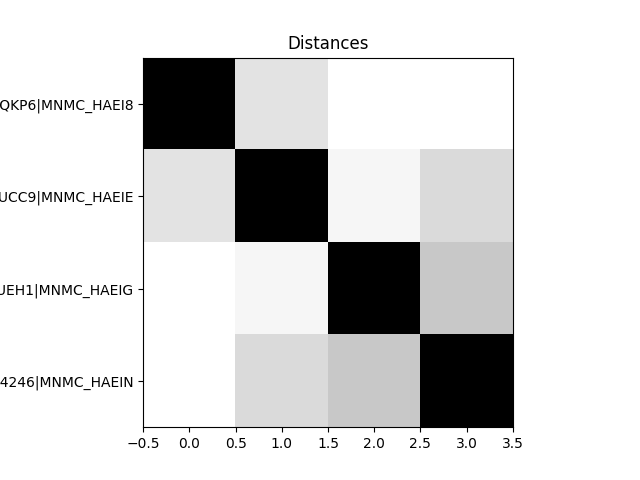
\includegraphics[width=0.8\textwidth]{poisson.png}

\section{Exercise 7: Curate the MalS.fa dataset}

Selected 31 sequences. Code:

\begin{minted}[linenos=false,fontsize=\small]{python}
import pandas as pd

def get_yeasts():
  """ Get a list of all the yeast species """
  df = pd.read_csv("Files_WS2/sugars.csv")
  return list(df["Yeast"])

def exercise_7():
  """ 
  Curate the MalS.fa dataset
  """

  # Get all yeast from sugars.csv
  yeasts = get_yeasts()

  mals = guide.readFastaFile('Files_WS2/MalS.fa', guide.Protein_Alphabet)
  cnt = 0
  select = []

  # traverse mals dataset
  for seq in mals:

    # we are only interested in yeast also in the sugars.csv list
    if seq.name in yeasts:

      # white space -> _
      new_name = (seq.name + "_" + seq.annot).replace(" ", "_")
      seq.name = new_name
      cnt += 1
      select.append(seq)

  guide.writeFastaFile('select.fa', select)
  print('Selected', cnt, 'sequences')
\end{minted}


\section{Exercise 8: Identify the consensus sequence for the MalS alignment}

I put my fasta file into the ClustaW web interface, and this is the consensus sequence it gave me.

\seqsplit{---MTISSAHPETEPKWWKEATIYQIYPASFKDSN-----------NDGWGDLKGIASKLEYIKELGVDAIWICPFYDSPQDDMGYDIANYEKVWPTYGTNEDCFALIEKTHKLGMKFITDLVINHCSSEHEWFKESRSSKTNPKRDWFFWRPPKGYDAEGKPIPPNNWRSFFGGSAWTFDEKTQEFYLRLFASTQPDLNWENEDCRKAIYESAVGYWLDHGVDGFRIDVGSLYSKVPGLPDAPVTDENSKWQHSDPFTMNGPRIHEFHQEMNKFMRNRV-KDGREIMTVGEVQHGSDETKRLYTSASRHELSELFNFSHTDVGTSPKFRYNLVPFELKDWKVALAELFRFINGTDCWSTIYLENHDQPRSITRFGDDSPKNRVISGKLLSVLLVSLTGTLYVYQGQELGQINF-KNWPIEKYEDVEVRNNYKAIKEEHGENSK---EMKKFLEGIALISRDHARTPMPWTKEEPNAGFSG---PDAKPWFYLNESFREGINAEDESKDPNSVLNFWKEALQFRKAHKDITVYGYDFEFIDLDNKKLFSFTKK--Y-DNKTLFAALNFSSDEIDFTIPNDSASFKLEFGNYPDKEVDASSRTLKPWEGRIYISE--}

\section{Exercise 9: Locate the MalS active site in the alignment}

Here is my approach:

\begin{enumerate}
    \item Find the sequence for the Ima1 protein in the dataset in Voordeckers et al. (2012)
    \item Look at the locations identified in the paper (see below image)
    \item Programmatically slice and inspect my alignment and find the (mostly) matching sequence
\end{enumerate}

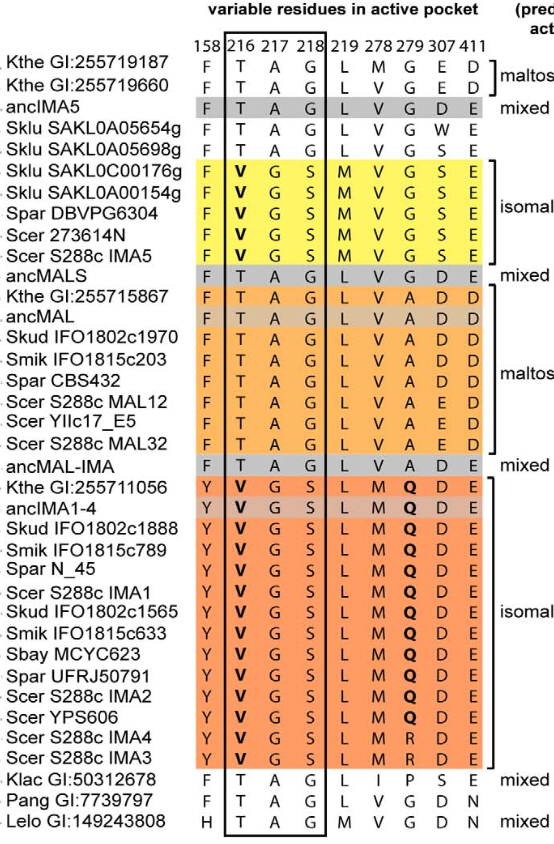
\includegraphics[width=0.8\textwidth]{residues.png}

\section{Exercise 10: Infer the phylogenetic relationships among select MalS proteins}

\begin{minted}[linenos=false,fontsize=\small]{python}
def exercise_10():
  aln = guide.readClustalFile('exercise7.aln', guide.Protein_Alphabet)
  phy = guide.runUPGMA(aln, 'poisson')
  print(phy) # print so we can copy into jstree 
  return phy
\end{minted}

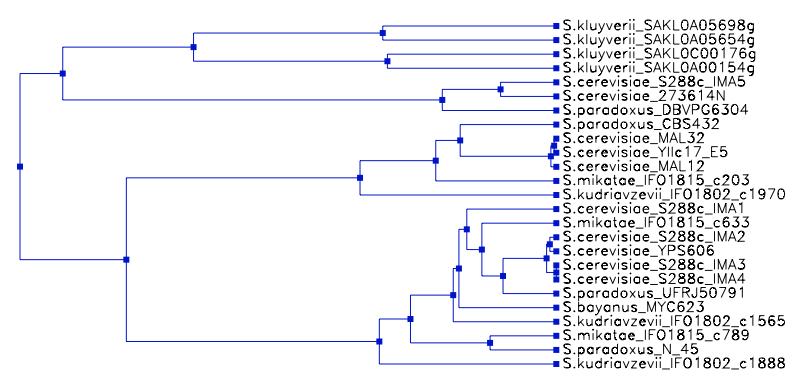
\includegraphics[width=0.8\textwidth]{tree.png}

TODO: I don't really understand what to do next.

\section{Exercise 11: Annotate your tree with metabolised sugars}

Here is my code. I loop each sugar, then for each one, loop each yeast and update the labels with string replacement.


I found Melizitose can metabolize => 8 / 14 sugars. I visualized it.

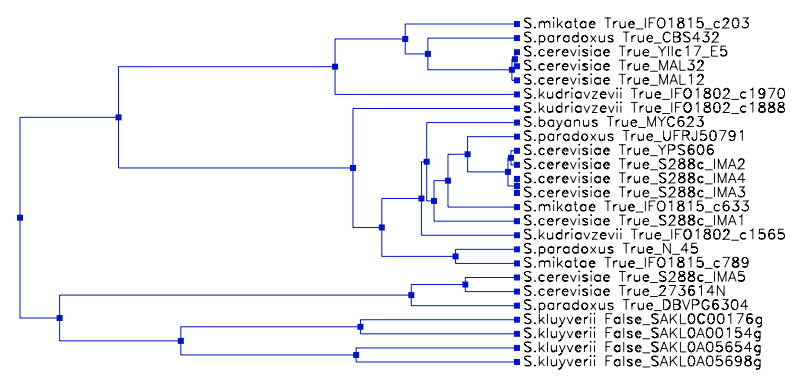
\includegraphics[width=0.8\textwidth]{tree2.png}

This tree suggests that at some point in the past, there was a speciation event and S.kluyverii diverged from the other Saccharomyces. At this split, S.kluyverii underwent a mutation(s) in a gene(s) and became unable to metabolize Melizitose.

Code:

\begin{minted}[linenos=false,fontsize=\small]{python}
def exercise_11():
  """ Annotate tree with metabolized sugars """
  df = pd.read_csv("Files_WS2/sugars.csv")
  yeasts = list(df["Yeast"])                        
  aln = guide.readClustalFile('exercise7.aln', guide.Protein_Alphabet)
  phy = guide.runUPGMA(aln, 'poisson')
  df = df.set_index(df['Yeast'])

  for col_name in df.columns[1:]:
    phy_copy = str(phy)
    t = 0
    f = 0
    for yeast in yeasts:
      can_metabolize = df[col_name][yeast]
      # add the labels using string replacement
      phy_copy = phy_copy.replace(yeast, f"{yeast} {can_metabolize}")
      # debugging - can see how many sugars can be metabolized
      if can_metabolize: 
        t += 1
      else:
        f += 1

    # Prints: <Melizitose> => 8 / 14 = 57.14285714285714
    # Useful for debugging
    print(f"{col_name} => {t} / {f + t} = {(t / (t + f)) * 100}")
\end{minted}

\section{Exercise 12: Identify the active sites at inferred ancestral sequences}

I don't really understand what to do here!

\end{document}